\chapter{Call Signatures Plugin}\label{chapter:plugin}
In \autoref{chapter:call signatures}, we introduced Call Signatures, patterns that describe function calls. In this chapter, we implement an IDA Pro plugin (discussed in \autoref{section:ida pro plugins}): \emph{Call Signatures Plugin} (CSP for short). The goal of CSP is to search for function calls that match Call Signatures in a binary. In other words, Call Signatures and CSP are complementary: Call Signatures describe function calls and CSP searches for these function calls in a binary.

In \autoref{chapter:experiments}, we experiment with this plugin by analyzing real-world world samples using Call Signatures from \autoref{chapter:call signatures for persistence techniques}.

\medskip

IDA Pro provides two advantages. First, IDA Pro contains a large suite of state-of-the-art static analysis tools, such as a disassembler and decompiler. IDA Pro plugins can build on these to automate part of malware analysis. Secondly, it allows malware analysts to easily integrate the plugin into their analysis routine, as many malware analysts will be using IDA Pro \cite{ida_guide}.

IDA Pro allows users to search for basic patterns (e.g. strings and bytes), but not for more complex structures (e.g. function calls). To search for specific structures or patterns, users need to implement their own plugin.

\medskip

The source code is available at \url{https://github.com/joren485/CallSignaturesPlugin}.

\medskip

The analysis of a binary using CSP is done in the following steps:
\begin{enumerate}
    \item Before the plugin runs, IDA Pro disassembles the binary and extracts useful information. One of the most important steps the disassembler takes is to deduce the boundaries of each function in the binary.

    \item CSP reads all Call Signatures (i.e. YAML files) in the plugin directory.

    \item CSP loops over each function that IDA Pro has detected. For each function it takes the following steps:
    \begin{enumerate}
        \item If IDA Pro detects that the function matches a F.L.I.R.T. signature (see \autoref{chapter:related work}), the function is skipped and CSP continues with the next function in the binary.

        Functions that match F.L.I.R.T. signatures are known uninteresting functions. They are either library functions (e.g. functions from the C standard library) or external functions (e.g. functions from a DLL). We skip these because we are interested in the functionality of the binary, not in the functionality of functions from libraries used by the binary.

        \item CSP instructs IDA Pro to decompile the function. This transforms the assembly instructions of the function into C-like pseudocode.

        Decompilation relies heavily on probabilistic heuristics because a lot of information is lost during compilation. Because of this, decompilation might fail, because the decompiler is unable to reconstruct assembly into pseudocode.

        This decompilation includes reconstructing function calls as we discussed in \autoref{section:decompiling function calls}.

        \item CSP compares each function call to each Call Signature. This process is discussed in more detail in \autoref{section:matching function call call signatures}.

        If a function call matches a Call Signature, CSP writes to the IDA Pro log that a match was found.
    \end{enumerate}
\end{enumerate}

\medskip

\autoref{fig:csp screenshot} shows a screenshot of IDA Pro after CSP analyzed a sample\footnote{\texttt{4c01ffcc90e6271374b34b252fefb5d6fffda29f6ad645a879a159f78e095979}}.
We can see an open tab that shows a list of detected function calls. For each function call, the plugin lists the address of the call instruction, the persistence technique, the decompiled call and the Call Signature that matched.

\begin{figure}[ht]
    \centering
    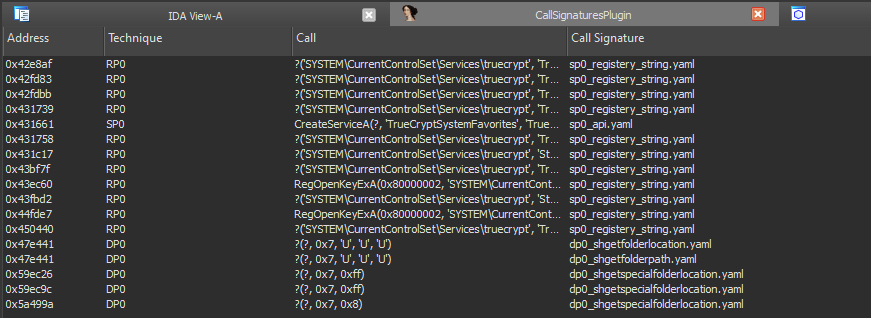
\includegraphics[width=\textwidth]{resources/images/csp_screenshot.png}
    \caption{A screenshot of CSP.}
    \label{fig:csp screenshot}
\end{figure}

\section{Call Signature Matching}\label{section:matching function call call signatures}
For a function call to match a Call Signature, each of the rules in the Call Signature should succeed.

As discussed in \autoref{section:call signature rules}, a rule is a constraint on a function call element (e.g. the function name). A rule can either succeed (i.e. the values match) or fail (i.e. the values do not match).

CSP iterates through each rule in a Call Signature and compares the constraint in the rule with the value of the relevant function call element.

The values of function call elements are often unknown, as information is lost during compilation (e.g. function names are not available in binaries) or determined at runtime (e.g. arguments passed by reference). Whether the value of the function call element is known, determines how the rule is applied to the function call element. The matching algorithm covers multiple situations:
\begin{itemize}
    \item If the rule specifies a constraint on a value and the function call element value is known, the values are compared using the operator specified in the rule.

    \item If the rule specifies a constraint on a type and the function call element value is known, the rule succeeds if the type of the function call element value equals the type specified in the rule.

    \item If the function call element value is not known, the result depends on the function call element:

    \begin{itemize}
        \item If the function call element is the function name, the rule succeeds.

        Because the disassembler can often not determine which function is being called (e.g. because the call is indirect), the function name is frequently unknown. To prevent many false negatives with rules that define a constraint on the function name, the rule succeeds.

        \item If the function call element is a specific argument or any argument, the rule fails.

        The decompiler will not be able to determine the value of the majority of arguments passed in function calls (most often because the value is computed at runtime). To prevent too many false positives, the rule fails if the argument value is unknown.
    \end{itemize}
\end{itemize}

\section{Examples of Call Signatures Matching}\label{section:examples searching function calls using Call Signatures}
In this section, we will look at an example of matching a function calls and Call Signatures. This is an example of the process laid out in \autoref{section:matching function call call signatures}.

In this example, we will use an example function (\autoref{listing:sum function plugin}) and corresponding Call Signature \autoref{listing:call signature sum plugin} from \autoref{section:call signatures examples}

\begin{lstlisting}[label={listing:sum function plugin}, caption={A C function that adds two integers.}, captionpos=b]
int sum(int a, int b){
    return a + b;
}
\end{lstlisting}

\begin{lstlisting}[label={listing:call signature sum plugin}, caption={A Call Signature for \texttt{sum}.}, captionpos=b]
---

signature:
    technique: "AddSum"
    description: >
        This Call Signature can be used to
        search for calls to sum.
    rules:
        - element: "function name"
          equals: "sum"

        - element: "number of arguments"
          equals: 2

        - element: "argument"
          argument_index: 0
          type: "number"

        - element: "argument"
          argument_index: 1
          type: "number"

        - element: "any argument"
          equals: 10
\end{lstlisting}

\medskip

Let's say that IDA Pro identified the following function calls in a binary. To see if any of them match the Call Signature in \autoref{listing:call signature sum plugin}, we need to iterate through all the rules and see if they succeed when applied to the function call. In the following examples, a ``?'' signifies a function call element with an unknown value.
\begin{itemize}
    \item \texttt{sum(2, 3)}
    \begin{enumerate}
        \item The first rule succeeds because the function name equals ``\texttt{sum}''.

        \item The second rule succeeds because the call takes two arguments.

        \item The third rule succeeds because the first argument is an integer (i.e. a number).

        \item The fourth rule succeeds because the second argument is also an integer.

        \item The fifth rule fails, because no argument is equal to 10.
    \end{enumerate}

    As the fifth rule failed, this call is not a match.

    \item \texttt{?(5, 10)}
    \begin{enumerate}
        \item The first rule succeeds, as the function name is allowed to be unknown. This is explained in detail in \autoref{listing:call signature sum plugin}.

        \item The second rule succeeds because the call takes two arguments.

        \item The third rule succeeds because the first argument is an integer.

        \item The fourth rule succeeds because the second argument is also an integer.

        \item The fifth rule succeeds because an argument (i.e. the second argument) is equal to 10.
    \end{enumerate}

    As all rules succeeded, this call is a match for the Call Signature in \autoref{listing:call signature sum plugin}.

    \item \texttt{sum(10, ?)}
    \begin{enumerate}
        \item The first rule succeeds because the function name equals ``\texttt{sum}''.

        \item The second rule succeeds because the call takes two arguments.

        \item The third rule succeeds because the first argument is an integer.

        \item The fourth rule failed, because the second argument is unknown. Unlike, the function name, rules will always fail on unknown arguments. This is explained in detail in \autoref{listing:call signature sum plugin}.
    \end{enumerate}

    As the fourth rule failed, this call is not considered a match and the fifth rule is not applied.
\end{itemize}

